\documentclass{article} 

% if you need to pass options to natbib, use, e.g.: 
% 	\PassOptionsToPackage{numbers, compress}{natbib} 
% before loading neurips_2018 

% ready for submission 
% \usepackage{neurips_2018} 

% to compile a preprint version, e.g., for submission to arXiv, add add the 
% [preprint] option: 
% 	\usepackage[preprint]{neurips_2018} 

% to compile a camera-ready version, add the [final] option, e.g.: \usepackage[final]{nips_2018}
 
% to avoid loading the natbib package, add option nonatbib: 
% 	\usepackage[nonatbib]{neurips_2018} 

\usepackage[utf8]{inputenc} % allow utf-8 input 
\usepackage[T1]{fontenc} % use 8-bit T1 fonts 
\usepackage{hyperref} % hyperlinks 
\usepackage{url} % simple URL typesetting 
\usepackage{booktabs} % professional-quality tables 
\usepackage{amsfonts} % blackboard math symbols 
\usepackage{nicefrac} % compact symbols for 1/2, etc. 
\usepackage{microtype} % microtypography
\usepackage{lmodern}
\usepackage{float}
\usepackage{graphicx}
\usepackage{subfig}
\usepackage{hyperref}
 
\title{SGDBabysitter} 

% The \author macro works with any number of authors. There are two commands 
% used to separate the names and addresses of multiple authors: \And and \AND. 
% 
% Using \And between authors leaves it to LaTeX to determine where to break the 
% lines. Using \AND forces a line break at that point. So, if LaTeX puts 3 of 4 
% authors names on the first line, and the last on the second line, try using 
% \AND instead of \And before the third author name.

\author{
	\begin{tabular}{rl}
			Joshua Catalano &|  28675650 \\
		Puranjay Rohan Gulati &|  96579164
	\end{tabular}
% examples of more authors % \And % Coauthor \\ % Affiliation \\ % Address \\ % \texttt{email} \\ % \AND % Coauthor \\ % Affiliation \\ % Address \\ % \texttt{email} \\ % \And % Coauthor \\ % Affiliation \\ % Address \\ % \texttt{email} \\ % \And % Coauthor \\ % Affiliation \\ % Address \\ % \texttt{email} \\ 
}

 \begin{document} 
 %\nipsfinalcopy is no longer used 
 \maketitle 
 
 \begin{abstract} 
 	We created a stochastic gradient descent algorithm that dynamically adjusts learning rate and batch size. To make decisions, the algorithm considers the change in validation error over time and the angle between gradients. We have exploited our knowledge of the behavior of stochastic gradient descent in order to create an implementation that attains lower validation errors. We consider our algorithm a success if it can attain a lower validation error than the best algorithms using constant learning rates or learning rates determined by a predetermined series of numbers (e.g. $\frac{1}{t}$ or $\frac{1}{\sqrt{t}}$). In this work, we have tested our algorithm against constant learning rate mini-batch gradient descent. For testing, we use the algorithms to fit a basic deep neural network to various real and generated datasets. Our code can be found on GitHub at \url{https://github.com/JayCata/SGDBabysitter.jl}
\end{abstract} 

\section{Introduction}  
%As we learned in class, 
\par Stochastic Gradient Descent (SGD) is a popular optimization algorithm in machine learning that allows for fitting various models to massive datasets. It can be used to fit logistic regression, ordinary least squares, neural networks, and more. While SGD is less computationally costly than gradient descent, it demonstrates unsavory behavior due to the fact that it assesses the gradient using a random subsample of the data. We constructed our own unique implementation that accounts for this strange behavior in the hopes of improving the performance of models that are fit using SGD. 
\par Making an implementation of stochastic gradient descent that provides more accurate estimates of the minima is important because it could improve the accuracy of existing models. Since many academic disciplines and the private sector use SGD to fit machine learning models, such improvements could result in better prediction performance in all types of applications. In addition, our implementation also has the benefit of not requiring `babysitting' to obtain low validation errors - resulting in less investment of time and knowledge from the end user. 

\section{Related Work}
\par A substantial amount of work has been done to improve gradient descent optimization algorithms for minimizing neural network loss functions. SGD with mini-batches combines fast optimization characteristic of SGD with the lower variance of regular batch gradient descent by computing the gradient for a fixed subset of the training examples (usually under 512 at a time) $ [1] $. However, this requires selection of the appropriate learning rate and batch size for the given dataset, which is a non-trivial task, to say the least. In comparison, algorithms that attempt to reduce the learning rate $ [2] $ to `anneal' closer to the minima can obtain better estimates of the best set of parameters. However, since loss functions in neural networks are, in general, non-convex, this often leads to minima that are not ideal since the gradient descent algorithm is still going down a single path. SGD with restarts $ [3] $ addresses this problem by suddenly increasing the learning rate after decreasing gradually in order to allow the algorithm to `jump' out of bad local minima and saddle points $ [4] $ and find better minima. However, this too requires prior selection of the learning rate schedule and makes no attempt to select appropriate mini-batch sizes. 
\par We have tried to address the limitations of these methods by creating a dynamic simultaneous learning rate and mini-batch size schedule which selects these hyperparameters on the basis of validation error, while also allowing for restarts when the error stagnates. 
\par However, many more algorithms exist that address the limitations of the aforementioned methods, albeit by different means. Algorithms such as Nesterov accelerated gradient, Adagrad, RMSprop, Adam, etc. use information about previous gradients and different learning rates for individual parameters to improve converge to minima. They have been found wide application in neural networks and work particularly well with sparse data sets $ [5] $. 


\section{Theory} 

\par In order to create this algorithm, we utilized the concepts we learned in class. In this section, we will discuss our understanding of the theory. 
\par When far away from the minimizer, stochastic gradient descent, with an appropriate learning rate, moves us closer to the minimizer with high probability. As it gets closer to the minimizer, the angles between the gradients assessed at all the different values of X become wider and wider. This increases the probability that the next iteration will actually move away from the minimizer. In class, we called this phenomenon the ``region of confusion.''
\par By decreasing the learning rate as we enter this region, we can potentially restrict how much the region of confusion pushes us away from the true minimizer. Starting with a very tiny learning rate, however, can make the algorithm take far too long to converge. On the other hand, having too large of a learning rate can give you divergent results. Thus, ideally, the learning rate would be large in the beginning but just small enough so that the algorithm doesn't diverge. Then as we approach the minimizer, this learning rate should decay so that we can get closer to the minimizer within the region of confusion. 
\par When selecting batch size, the trade-off is between lower computation costs and a more accurate estimate of the gradient. When far away from the minimizer, a small batch size is ideal because the angle between the gradients evaluated at any of the X values should be relatively small, so taking an average of gradients is less beneficial but still increases computation cost. As we approach the minimizer, the angles between these gradients increase, and averaging will be more beneficial as more gradients are likely to be pointing in the wrong direction. 
\par Our algorithm tries to take this theory in mind. To initialize step size, we run ten iterations of constant, vanilla gradient descent to see if those ten iterations decreased validation error by a certain amount. If so, we use that as our initial step size. If not, we decrease the step size and run another ten iterations. When the algorithm is running after initialization, every fixed number of iterations, we check the validations error and half as frequently, we run our logic that selects new step sizes and batch sizes based on the angle between gradients and the change in validation error.

\section{Analysis}
\subsection{Tests on Simulated Data}
We applied our SGD algorithm and the Neural Network to a problem in econometrics. When estimating parameters using linear regression, economists are frequently interested in interpreting the coefficients as the effect of one variable on another. Missing data can be a problem for such an interpretation. If data is missing at a random, then there is no issue and you can just run regression on data that is not missing with no fear of bias in your estimated coefficients. On the other hand, if data is systematically missing, excluding it will cause these estimates to be biased.  In these circumstances, it may be worth imputing data (i.e. filling in the missing values) with machine learning techniques. 
\par In order to assess the effectiveness of these techniques, we must generate the data ourselves, so we can know the true parameters of what we are investigating and which technique is the most effective. 
For part of our testing, we generate data X1 and X2 by drawing from a normal distribution. Then we generate X3 by setting it equal to X1 and X2 plus some random unobserved error. We do this in order to establish some causal relationship between X3 and X1/X2.  Then we choose a specification for y, the dependent variable of interest. In this circumstance, we chose $y=2X1-3X2+4X3 +\epsilon$ where epsilon is some normally distributed error term.  In this specific circumstance, the parameters of interest are 2,-3, and 4. The closer we can get to these numbers, the better the machine learning technique is for data imputation. 
After generating the data, we run OLS on it to make sure everything is working properly, and we get estimates that are very close to [-2 3 4]. Next, I simulate the removal of data by looping through each example and removing approximately 50\% of examples that meet certain criteria.   We run OLS on the non-missing data to show the bias this introduces into the estimates. We then train a neural network on the data that is not missing using a vanilla SGD implementation and our SGDBabysitter implementation.  
\par We use these trained weights to predict on the missing data. We then fill in the missing values with these predicted values and run OLS on all of the data (both examples that had missing values and those that did not) to obtain two sets of coefficients, one from the vanilla implementation and one from ours.  We run this simulation five times and obtain the following relatively positive results:
True Coefficients: [2,-3,4] \newline
All Data Coefficients: [1.99537, -2.99519, 3.99441] \newline
Coefficients with Missing Data:[2.06545, -3.1007, 4.13595] \newline
Coefficients with NN Imputation (SGDBabysitter): [1.99037, -3.08193, 4.11074]\newline Coefficients with NN Imputation (VanillaSGD): [1.94844, -3.10303, 4.12519]

\subsection{Tests on Real Data}
To further test our algorithm, we compared it to a vanilla implementation of mini-batch SGD on various real datasets. However, we first ran a hyperparameter search in order to the find the hyperparameters which gave the best validation error for each dataset. In order to avoid overfitting and for consistent results, we chose a $ 4 $-layer neural network with layer sizes of $ 3, 3, 4, $ and $ 3 $ respectively for all datasets prior to testing.
\\

%\begin{flushleft}
\textbf{MNIST Data Set}
%\end{flushleft}
\par On the MNIST database of handwritten digits $ [6] $, 
%we employed a neural network with 4 four hidden layers of size $ 3, 3, 4, $ and $ 3 $ respectively. 
we consistently performed better than the vanilla implementation. Plots of sum of squared errors versus SGD iterations shows the performance of the two algorithms. Whereas regular SGD seems to consistently find the same local minimum, our algorithm is able to find a better minimum, and that too faster. Although our algorithm encourages looking for a better minimum when the validation error is stagnating, it is unable to find one. On other runs, we found that the vanilla implementation consistently plateaued at similar validation errors, however, our implementation mostly found the minimum with the sum of squared errors of $ \approx 4 $. We further ensured that we were not converging to a saddle point, a known issue with SGD algorithms that do not employ a momentum-like term $ [4] $, by looking at the resulting predictions.
\begin{figure}[H]
	\centering
	\subfloat[VanillaSGD]{{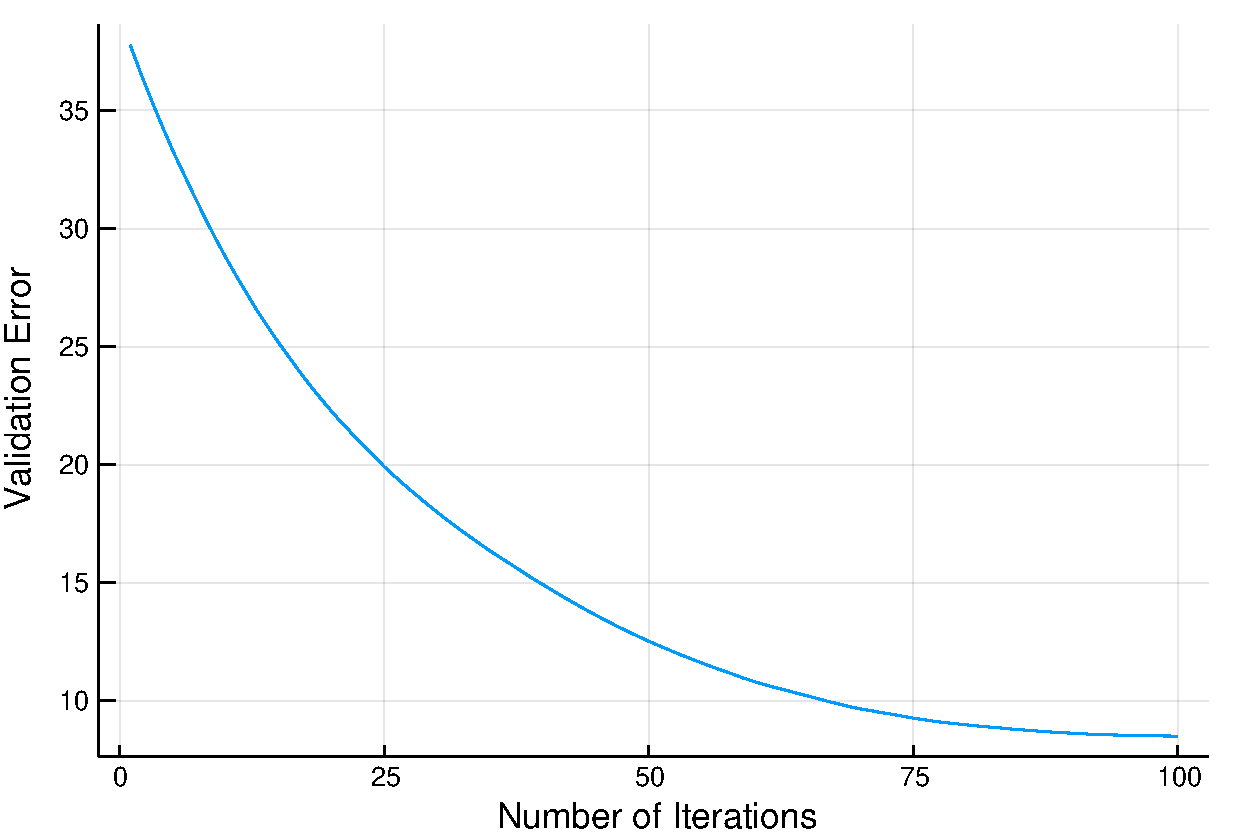
\includegraphics[width=5.5cm]{../figs/Vanilla_MNIST.pdf} }}%
	\quad
	\subfloat[SGDBabysitter]{{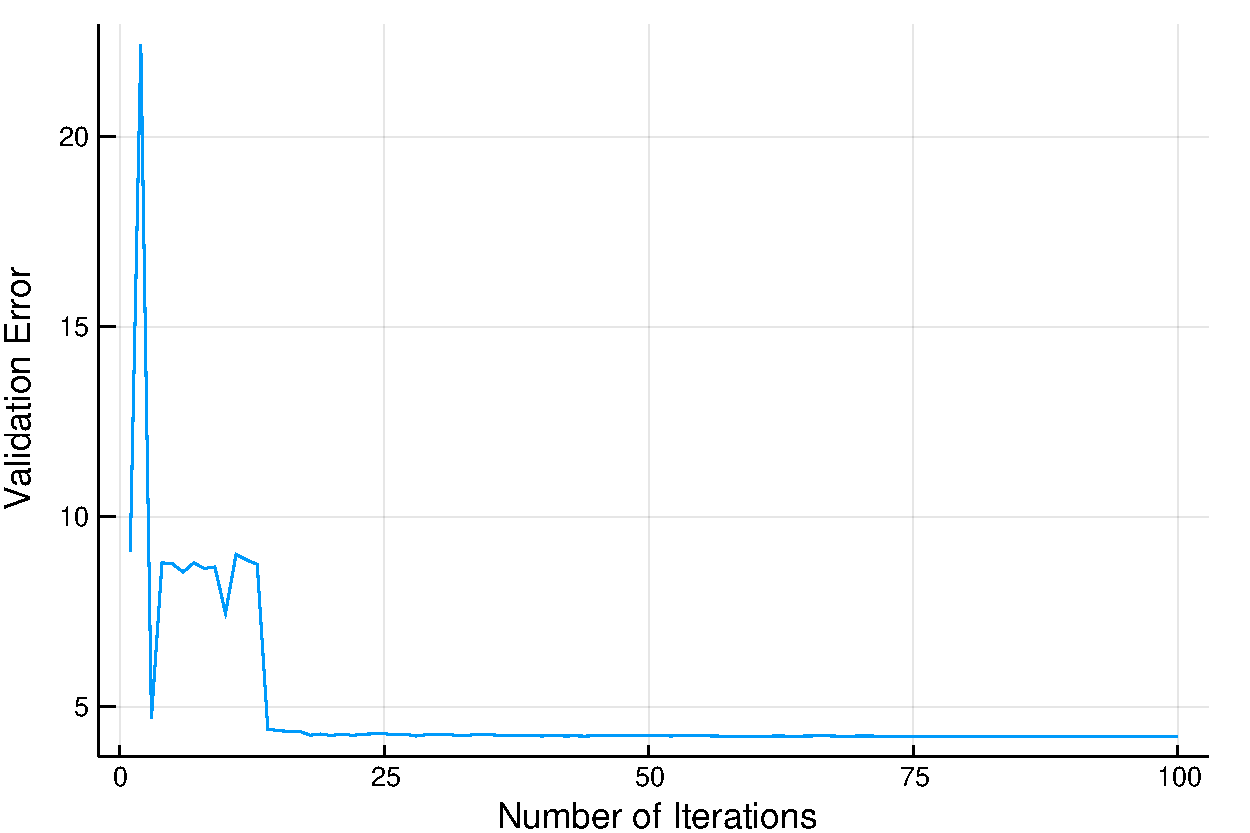
\includegraphics[width=5.5cm]{../figs/SGDB_MNIST.pdf} }}%
	\caption{Validation errors on MNIST data set}%
	\label{MNIST}%
\end{figure}

\textbf{Parkinsons Telemonitoring Data Set}
\par Next, we employed the Oxford Parkinson's Disease Telemonitoring dataset $ [7] $. We found similar validation errors for both the vanilla and babysitter implementations. However, vanilla SGD struggled to find the minima, with some peaks in the validation error, whereas our implementation found it much faster.
\begin{figure}[H]
	\centering
	\subfloat[VanillaSGD]{{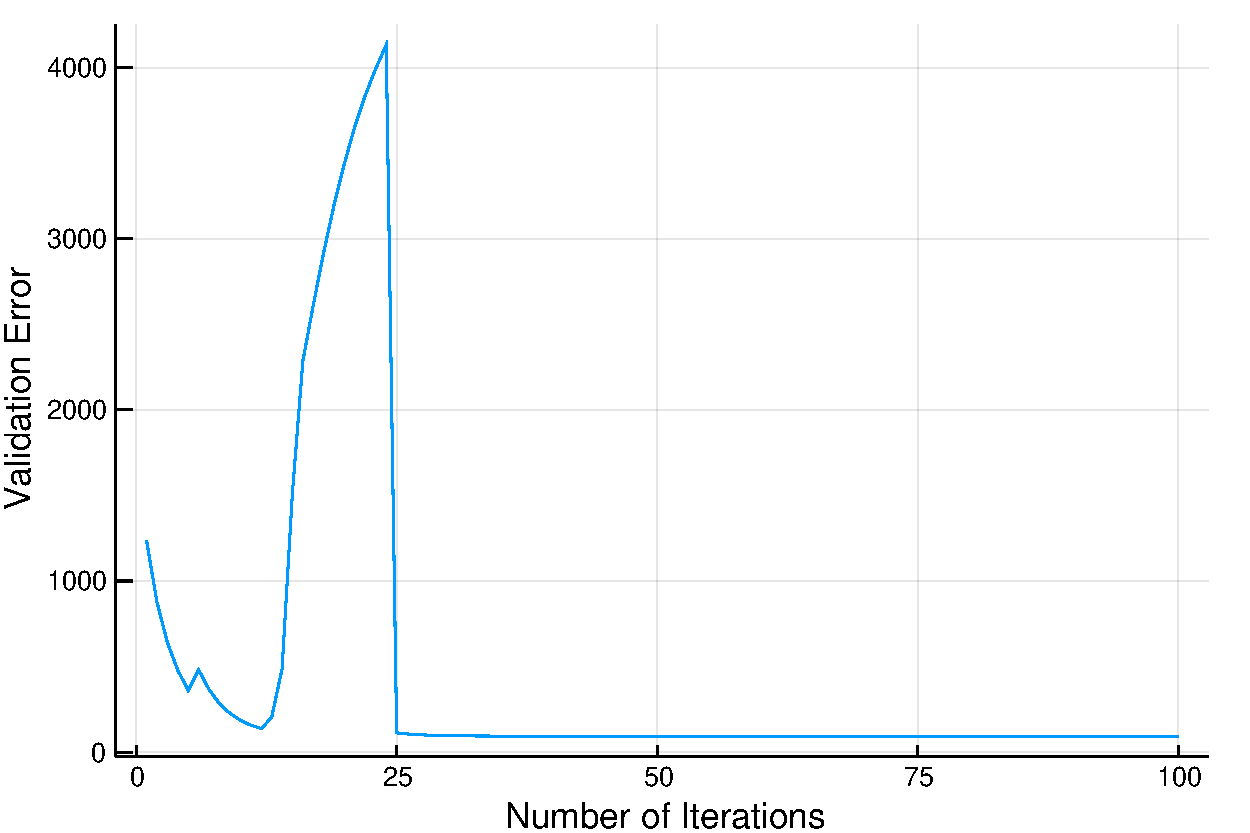
\includegraphics[width=5.5cm]{../figs/Vanilla_Parkinsons.pdf} }}%
	\quad
	\subfloat[SGDBabysitter]{{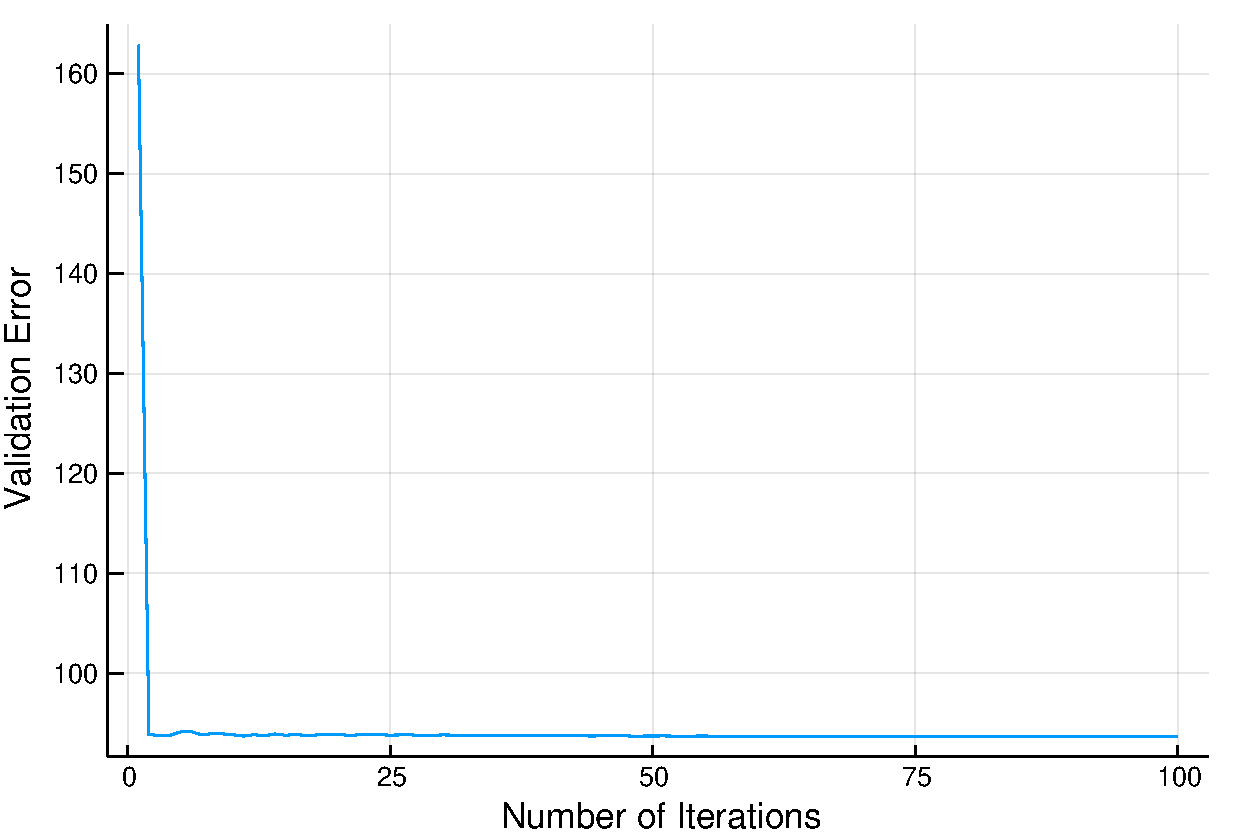
\includegraphics[width=5.5cm]{../figs/SGDB_Parkinsons.pdf} }}%
	\caption{Validation errors on Parkinson's telemonitoring data set}%
	\label{Parkinsons}%
\end{figure}

\textbf{Concrete Compressive Strength Data Set}
\par This dataset $ [8] $ aims to predict the compressive strength of concrete -  a highly non-linear function of various features - which is an important quantity for civil engineering applications. Based on our tests, we again found that SGDBabysitter and the vanilla implementation both consistently found the same minimum with comparable validation errors. 
\begin{figure}[H]
	\centering
	\subfloat[VanillaSGD]{{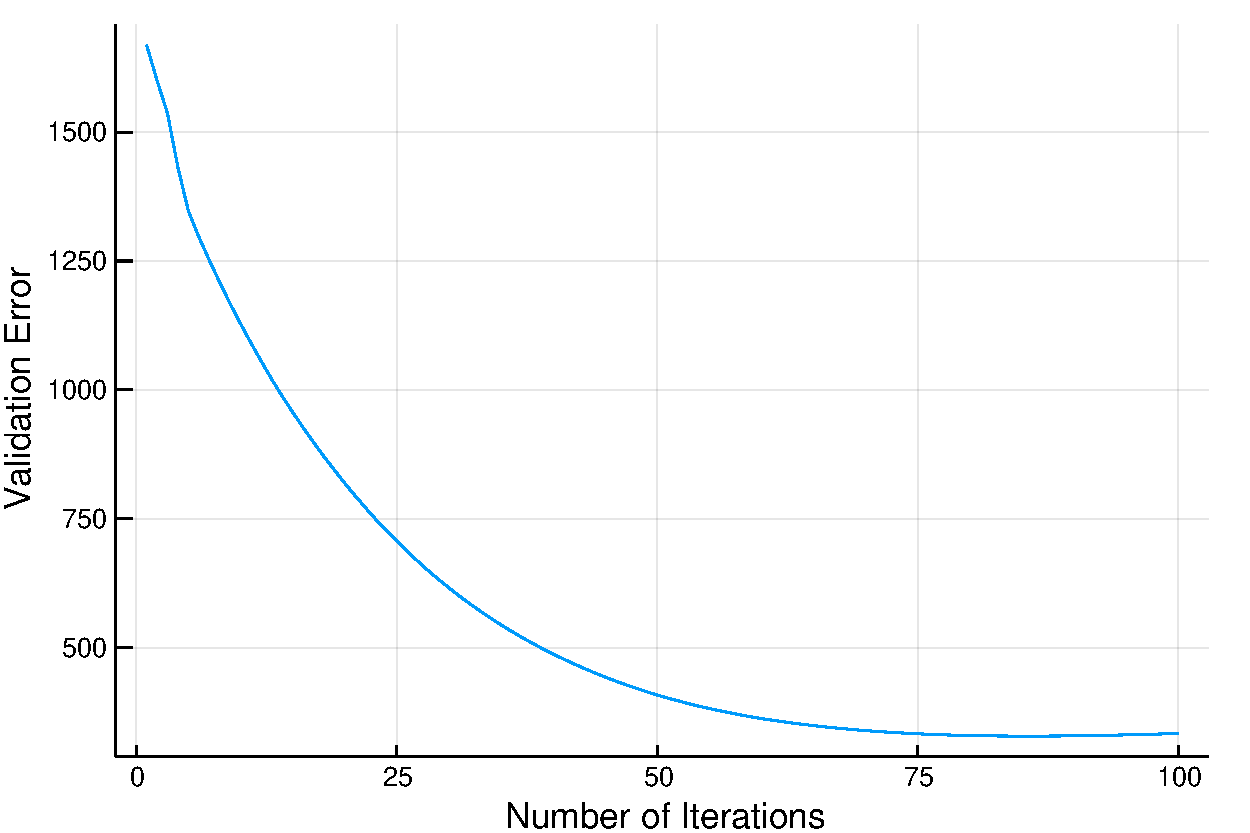
\includegraphics[width=5.5cm]{../figs/Vanilla_Concrete.pdf} }}%
	\quad
	\subfloat[SGDBabysitter]{{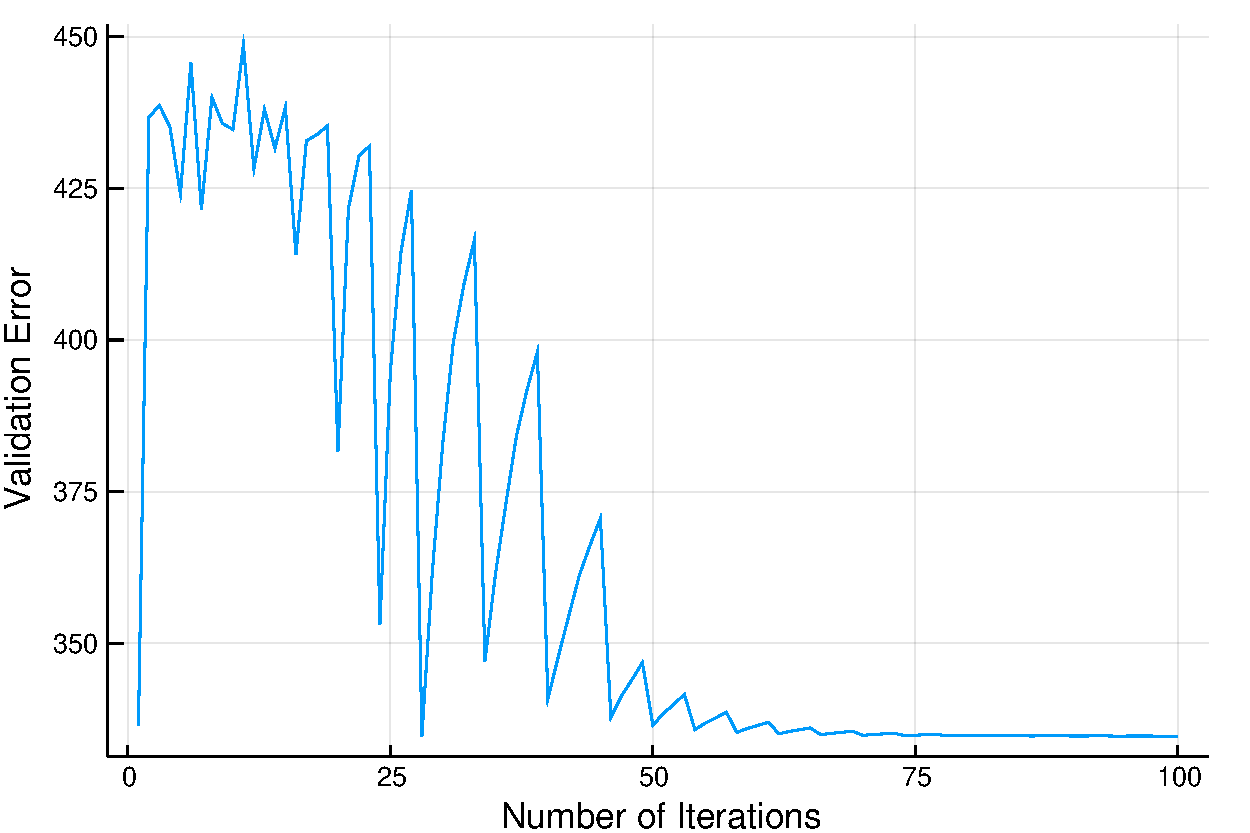
\includegraphics[width=5.5cm]{../figs/SGDB_Concrete.pdf} }}%
	\caption{Validation errors on the concrete data set}%
	\label{Concrete}%
\end{figure}
%\begin{figure}[H]
%	\includegraphics[width=.4\linewidth]{.Vanilla_Concrete2.pdf}
%	\label{Vanilla_Conc}
%\end{figure}
%\begin{figure}[H]
%	\includegraphics[width=.4\linewidth]{SGDB_Concrete2.pdf}
%	\label{SGDB_Conc}
%\end{figure}

\textbf{Discussion}
\par SGDBabysitter consistently performs better or on par with the vanilla implementation based on our tests with real data. However, we do believe that all $ 3 $ tests are not equally reliable estimators of performance, with the MNIST dataset providing the most trustworthy results. This is because the Parkinsons dataset had a large number of features which may have been irrelevant, and both the Parkinsons and concrete dataset were generally unclean with missing values. We were unable to clean both datasets or employ feature selection prior to testing due to time constraints. 

\section{Conclusions}
\par Based on the results above, our SGD babysitter generally provides performance better than vanilla mini-batch SGD. No time investment is required to find the ideal hyperparameters which can significantly reduce computation costs when using large datasets, and our initialization method gets us closer to minima much faster on all datasets. Further, reduced reliance on the end user for hyperparameter selection makes SGD babysitter comparatively easier to use and more robust over a wide range of applications. 

\par However, we do not feel that our limited testing is sufficient to conclusively show that our algorithm is objectively better. Further testing and logic improvements are required to make our algorithm an improvement over the vanilla implementation, which is abundantly used to this day. We do plan to continue working on our algorithm in the coming term.
 
\newpage
\section{References}

[1] Ruder, Sebastian. 2016. “An Overview of Gradient Descent Optimization Algorithms.” CoRR abs/1609.04747. http://arxiv.org/abs/1609.04747. \newline \newline
[2] Bottou, Leon. n.d. “Stochastic Gradient Learning in Neural Networks.” http://citeseerx.ist.psu.edu/viewdoc/download?doi=10.1.1.52.361
\newline \newline
[3] Loshchilov, Ilya, and Frank Hutter. 2016. “\{SGDR:\} Stochastic Gradient Descent with Restarts.” CoRR abs/1608.03983. http://arxiv.org/abs/1608.03983.
\newline \newline
[4] Dauphin, Yann, Razvan Pascanu, Çaglar Gülçehre, Kyunghyun Cho, Surya Ganguli, and Yoshua Bengio. 2014. “Identifying and Attacking the Saddle Point Problem in High-Dimensional Non-Convex Optimization.” CoRR abs/1406.2572. http://arxiv.org/abs/1406.2572.
\newline \newline
[5] Dean, Jeffrey, Greg S Corrado, Rajat Monga, Kai Chen, Matthieu Devin, Quoc V Le, Mark Z Mao, et al. 2012. “Large Scale Distributed Deep Networks.” In NIPS.
\newline \newline
[6] Lecun, Y, L Bottou, Y Bengio, and P Haffner. 1998. “Gradient-Based Learning Applied to Document Recognition.” Proceedings of the IEEE 86 (11): 2278–2324. https://doi.org/10.1109/5.726791.
\newline \newline
[7] Tsanas, A, M A Little, P E McSharry, and L O Ramig. 2010. “Accurate Telemonitoring of Parkinson’s Disease Progression by Noninvasive Speech Tests.” IEEE Transactions on Biomedical Engineering 57 (4): 884–93.\\ https://doi.org/10.1109/TBME.2009.2036000.
\newline \newline
[8] Yeh, I.-C. 1998. “Modeling of Strength of High-Performance Concrete Using Artificial Neural Networks.” Cement and Concrete Research 28 (12): 1797–1808. https://doi.org/https://doi.org/10.1016/S0008-8846(98)00165-3.
\end{document}
